% Generated from ../chapters/15-the-distribution-of-ages.md
\chapter{Chapter 15 --- The Distribution of Ages}\label{chapter-15-the-distribution-of-ages}

Chronological age assigns one number to an entire person. Biological-age clocks improve on this by estimating age from biomarkers, but they still often compress a heterogeneous organism into a scalar.

A better framework begins with types of components and functions. Let \(k_i\) denote a class: retinal ganglion cells, circulating immune cells, osteocytes, muscle fibres, mitochondrial populations, vascular function, learning capacity, or another defined subsystem.

Define

\[
p(k_i,\tau\mid T)
\]

as the proportion of components of type \(k_i\) in a person of chronological age \(T\) whose \textbf{chronological component age} lies near \(\tau\). For blood cells, this distribution is concentrated at young ages because turnover is rapid. For many neurons, it includes ages close to the person's lifetime.

Now define

\[
q(k_i,b\mid T)
\]

as the distribution of \textbf{functional or biological age} \(b\) for type \(k_i\), estimated relative to a reference population. A 55-year-old can have vascular function resembling the population mean at 40, muscle power resembling 50, and an epigenetic estimate resembling 60. These values are model-dependent, not literal ages.

The whole organism is therefore represented not by one age but by a family of distributions:

\[
\mathcal{A}(T)=\{p(k_i,\tau\mid T),q(k_i,b\mid T)\}_{i=1}^{m}.
\]

This formulation separates three ideas that scalar biological age confuses:

\begin{enumerate}
\def\labelenumi{\arabic{enumi}.}
\tightlist
\item
  how recently components were produced;
\item
  how old they function relative to a population;
\item
  how well different subsystems remain coordinated.
\end{enumerate}

\begin{figure}
\centering
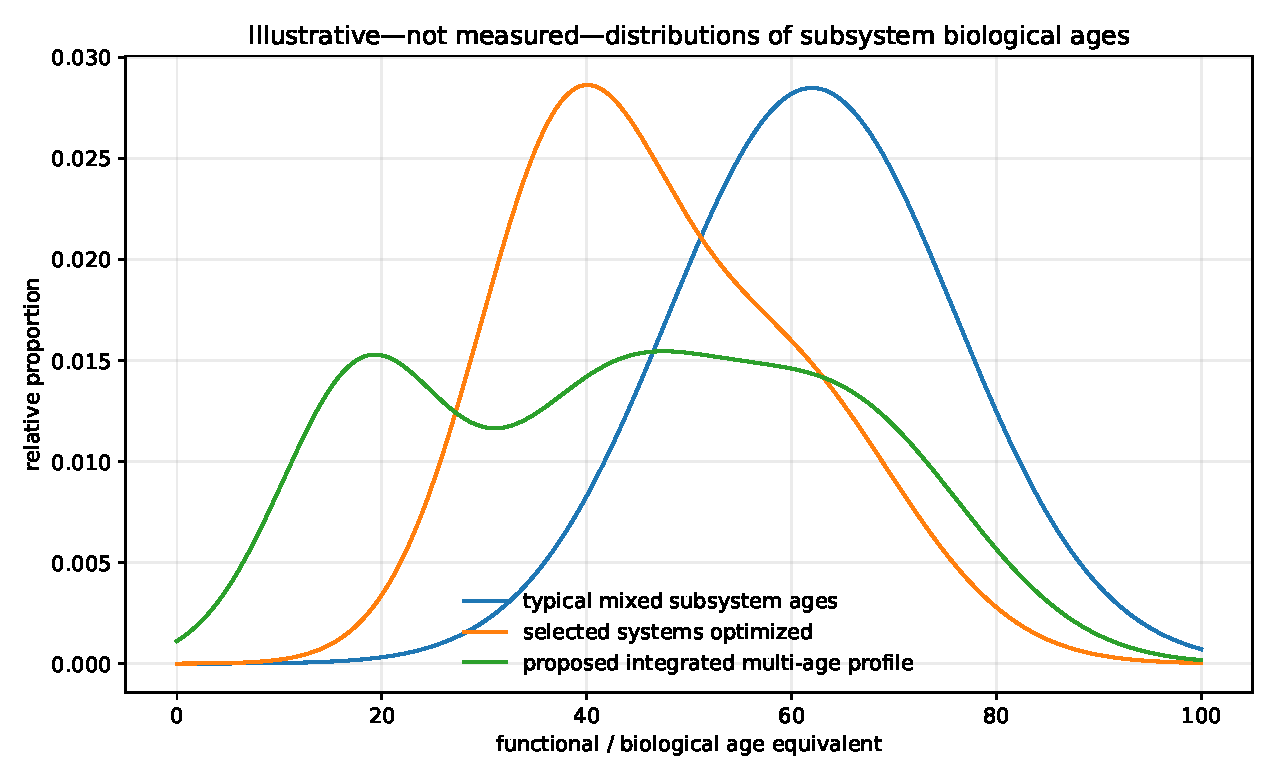
\includegraphics[width=0.9\textwidth]{../figures/age-distributions-v4.pdf}
\caption{Illustrative age distributions: ordinary aging broadens and shifts functional ages; optimized health may shift selected systems younger; the proposed ideal preserves renewal and coordination without forcing every component into the same age.}
\end{figure}

What is typical? In ordinary aging, fast-turnover populations remain chronologically young but may be produced by an aged niche and function poorly. Long-lived cells may be old chronologically yet healthy. Different clocks diverge.

What do quantified longevity practitioners show? Bryan Johnson, Siim Land, and high-level masters athletes report or demonstrate youthful values in selected dimensions---cardiorespiratory fitness, strength, blood pressure, body composition, metabolic markers, or pace-of-aging assays. The evidence supports \textbf{heterochrony}: different systems can occupy different functional ages. It does not justify assigning the entire person one youthful age.

What would the ideal distribution be in this framework? Not every component should become embryonic or infant-like. The aim is a coordinated mixture:

\begin{itemize}
\tightlist
\item
  rapid renewal where turnover is appropriate;
\item
  preservation of long-lived information-bearing cells;
\item
  youthful repair kinetics;
\item
  mature cognitive and social capacities;
\item
  continued access to play, learning, exploration, and developmental flexibility;
\item
  minimal accumulation of rigid, nonparticipating structure.
\end{itemize}

The ideal is therefore not uniform youth. It is \textbf{age diversity under coherent self-organization}. A person becomes a continuous integration of many ages rather than a failed attempt to freeze one age.

Parenthood and grandparenthood offer a behavioural example. Interaction with children reactivates carrying, crawling, imitation, play, touch, vocalization, teaching, protection, and wonder. These modes may reopen neural and bodily repertoires suppressed by adult routine. Claims of cellular rejuvenation would be premature, but the organism clearly becomes functionally multi-age.

This model generates research questions. Can age distributions be estimated across tissues? Does variation among subsystem ages predict resilience better than their mean? Does long-term practice reduce the oldest dysfunctional tail while preserving valuable long-lived structure? These are more informative questions than asking whether a person is ``biologically 37.''

\section{Why a mean age can mislead}\label{why-a-mean-age-can-mislead}

Suppose two people have the same average subsystem age. One has every system moderately old. The other has excellent cardiovascular and muscular function but severe degeneration in one critical organ. The average hides risk. Distribution shape, variance, and the oldest tail matter.

A useful summary might include

\[
\bar b=\sum_i w_i\int b\,q(k_i,b\mid T)\,db,
\]

but also a tail measure

\[
B_{\max,\alpha}=\text{upper }\alpha\text{-quantile of subsystem biological ages}.
\]

The weights \(w_i\) should reflect function and survival relevance, not convenience. These equations expose choices that commercial clocks often hide.

\section{Coordination age}\label{coordination-age}

A further variable is the age of coordination. Muscle, cardiovascular function, balance, and cognition may each look adequate alone but interact poorly under stress. The organism's effective age may depend on the weakest coupling among systems.

This motivates challenge tests rather than resting panels. A youthful system should coordinate and recover, not merely display youthful averages.
